\section{问题重述}\label{sec:problem-restatement}
\subsection{问题背景}

随着运动控制与环境感知技术的发展，四足机器人逐步应用于应急救援等场景，为代替人员进入复杂、危险环境开展作业提供了新的技术途径\cite{unitree-rescue}。\ref{fig:quadruped-field-debug}。

无线电干扰源的精准定位与清除需要在已确定的目标区域内完成。为使机器狗代替人员开展搜索，需依据有限的测向反馈规划检测位置、检测频道及清除顺序，在保证清除全部干扰源的前提下尽量缩短任务时间。目标区域为半径 $1800\,\mathrm{m}$ 的圆域，以圆心为原点，正东、正北分别为坐标轴正向。各干扰源占用互不相同且固定的频道，频道取自 $20$ 个已知频道，其有效接收半径为 $1000$ 至 $1500\,\mathrm{m}$；示向度误差在 $\pm1^\circ$ 内，同一地点重复检测不能消除该误差。

机器狗以 $5\,\mathrm{m/s}$ 沿直线移动，停下后才能检测。频道切换、一次检测、光学精确定位和清除分别耗时 $1$、$5$、$3$、$2\,\mathrm{s}$；距干扰源不超过 $20\,\mathrm{m}$ 时可进行光学精确定位和清除。任务总耗时由上述移动、换频、检测、光学定位及清除时间共同组成。

% 用户提供的前期实机调试照片；保留原图，不作为本文算法验证结果。
\begin{figure}[H]
\centering
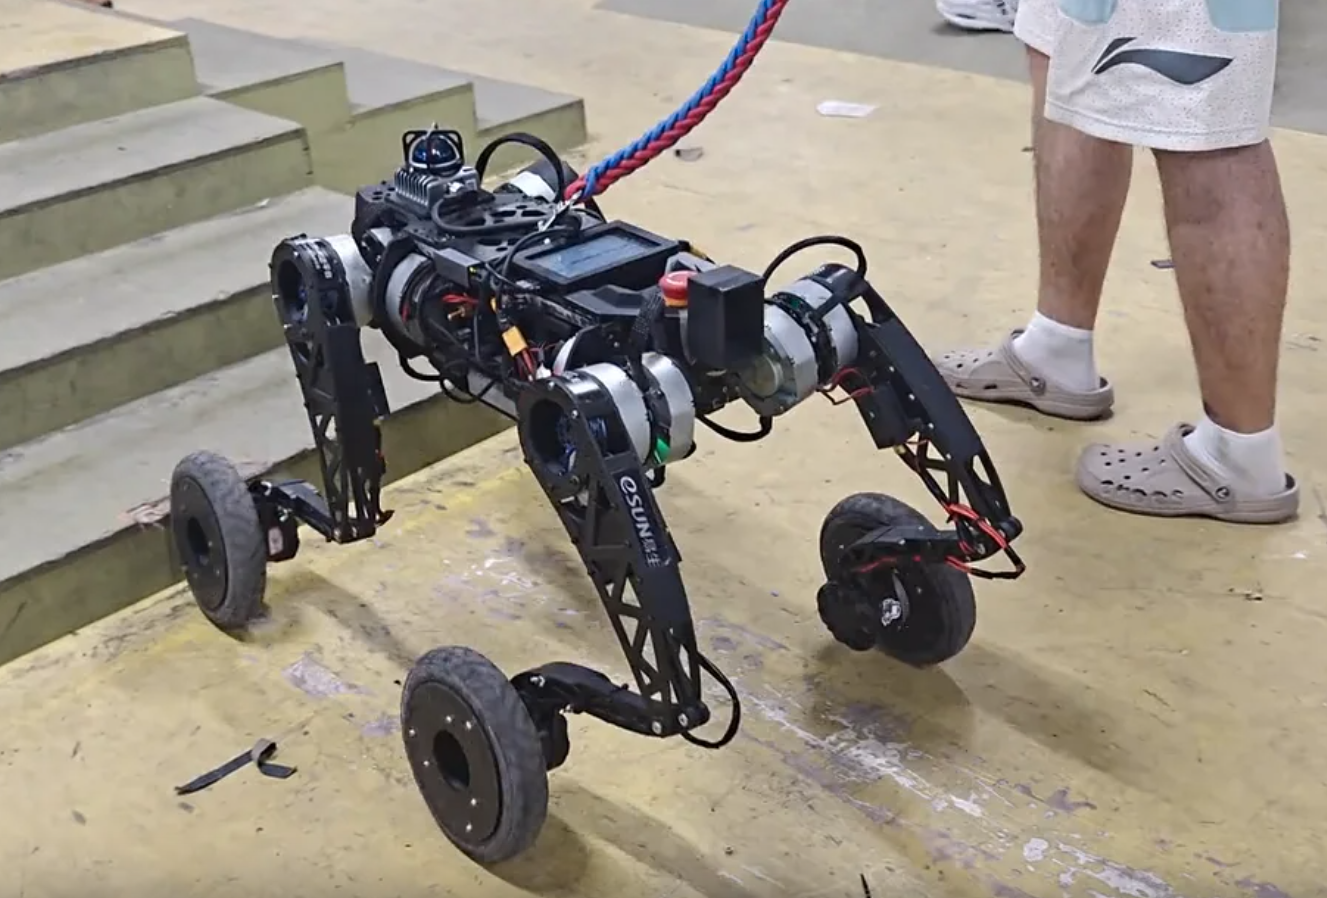
\includegraphics[width=0.64\linewidth,alt={轮式四足机器人示例。}]{figures/轮式四足机器人示例.png}
\caption{轮式四足机器人示例}
\label{fig:quadruped-field-debug}
\end{figure}

\subsection{问题要求}

\textbf{问题一：}根据多个检测点坐标及同一干扰源的示向度，给出采用交会定位法计算多边形定位区域直径的算法，并判断以该直径为直径的圆是否能够覆盖定位区域。

\textbf{问题二：}对于已在一个检测点测得示向度的全向干扰源，确定第二个检测点的选择策略及候选区域，以获得较好的定位效果。

\textbf{问题三：}目标区域内有 $10$ 至 $16$ 个全向干扰源，具体数量未知。机器狗从原点出发，测向机初始频道为 $1$，需制定自动搜索、定位与清除策略，使其在清除全部干扰源的前提下尽量减少总耗时。

\textbf{问题四：}在总数范围和初始条件不变的情况下，考虑全向与定向干扰源混合分布，且定向干扰源的数量及方向未知；定向源仅在发射方向两侧各 $90^\circ$ 内辐射信号，需据此制定检测与清除策略。

对问题三、四，均需通过演练检验清除比例和平均定位清除时间。清除比例为清除数与总数之比，平均定位清除时间为任务总耗时与清除数之比；并按题目要求分别报告三次正式测试结果及提供对应日志。

\clearpage
